\documentclass[compress]{beamer}

\usepackage{xeCJK}
%\usepackage[nofonts]{ctex}
\setCJKmainfont[ItalicFont={Kaiti SC}]{Kaiti SC}%
%\setCJKmainfont[ItalicFont={AR PL KaitiM GB}]{AR PL KaitiM GB}%
%\setCJKsansfont{WenQuanYi Zen Hei}% 文泉驿的黑体

\mode<beamer>
{
     \useinnertheme{rectangles}
     %\useoutertheme{infolines}
     %\useoutertheme{default}
     \usecolortheme{rose}
     \usecolortheme{seahorse}

     \setbeamertemplate{navigation symbols}{}%remove navigation symbols

     \expandafter\def\expandafter\insertshorttitle\expandafter{%
     \insertshorttitle\hfill%
     \insertframenumber\,/\,\inserttotalframenumber}
}

\mode<handout>
{
	\usetheme{default}
	\usepackage{pgfpages}
	\pgfpagesuselayout{4 on 1}[a4paper,landscape,border shrink=5mm]
}


\usepackage{amsmath,latexsym,amssymb,amsfonts,amsbsy}
\usepackage{ulem}
\usepackage{graphicx}
\usepackage{hyperref}
\usepackage{textpos}

\newcommand{\romannumber}[1]{{\textrm{\uppercase\expandafter{\romannumeral
#1}}}}

\graphicspath{{figure/}}

%%%%%%%%%%%%%%%%%%%%%%%%%%%%%%%%%%%%%%%%%%%%%%%%%%%%%%%%%%%%%%%%%
%    body                                                       %
%%%%%%%%%%%%%%%%%%%%%%%%%%%%%%%%%%%%%%%%%%%%%%%%%%%%%%%%%%%%%%%%%


\begin{document}

\AtBeginSection[]
{ 
    \begin{frame}<beamer> 
		\frametitle{内容提要} 
		\tableofcontents[currentsection,currentsubsection,
        subsectionstyle=show/shaded/hide] 
	\end{frame} 
} 

					
\title{面向对象的分析与设计\\ 教学计划}

\author[面向对象的分析与设计]
{曹东刚\\\href{mailto:caodg@pku.edu.cn}{caodg@pku.edu.cn}}

\institute[北京大学]{北京大学信息学院研究生课程}

\date{2017年2月-6月}

\titlegraphic{
\includegraphics[height=0.10\textwidth]{Overlays/logo.pdf}}

\begin{frame}
	\titlepage
\end{frame}

\setcounter{framenumber}{0}

\begin{frame}
  \frametitle{教材和课件}
\begin{thebibliography}{}
\bibitem{shao13}
   邵维忠, 杨芙清. 面向对象的分析与设计. 清华大学出版社, 2013年1月. ISBN: 978-7-302-30120-2
\end{thebibliography}

\begin{center}
  \centering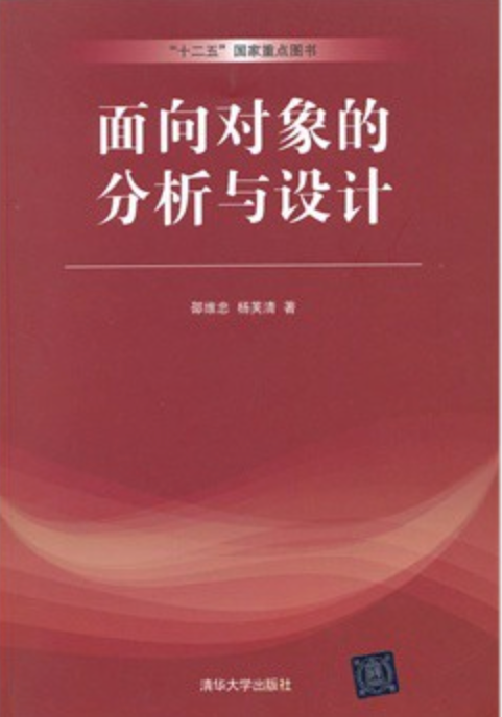
\includegraphics[height=3cm]{book.pdf}\hspace{1cm}%
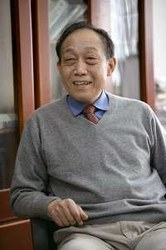
\includegraphics[height=3cm]{shao.jpg}%
\end{center}
\end{frame}


\begin{frame}
\frametitle{教学内容及学时 - 1}
\begin{block}{基础知识-9学时}
  讲述面向对象方法的基本概念及主要特点,分析比较各种建模方法,简要介绍
  UML及本书的OO方法概貌
\end{block}
\begin{block}{面向对象的分析OOA-12学时}
  通过研究问题域和用户需求,发现问题域中与系统责任有关的对象、对象的特征
  和相互关系。建立一个直接映射问题域,符合用户需求的OOA模型。
\end{block}
\end{frame}

\begin{frame}
\frametitle{教学内容及学时 - 2}
\begin{block}{面向对象的设计OOD-9学时}
  在OOA基础上,运用面向对象的概念与原则,按照具体的实现条件进行系统设计
  。产生一个可实现的OOD模型。
\end{block}

\begin{block}{新型开发技术-9学时}
  设计模式,新范型,新技术,新语言等
\end{block}

\begin{block}{专题研讨-6-9学时}
  技术报告,项目报告
\end{block}
\end{frame}

\begin{frame}
  \frametitle{平时作业}
  \begin{itemize}
    \item 每周课后布置
    \item 练习、作业
    \item 所有作业在线提交
    \item 要求独立完成, \uline{按时提交}, 延期成绩7折
  \end{itemize}
  作业网站: http://course.pku.edu.cn
\end{frame}

\begin{frame}
  \frametitle{大作业}
    用面向对象等方法完成一个小型系统的分析、设计与实现验证,并进行评价
  \begin{itemize}
    \item 需求描述与需求模型
    \item 系统分析模型
    \item 系统设计模型
    \item 实现验证
    \item 系统演化,调整设计与实现,重新验证
    \item 评价报告
  \end{itemize}
\end{frame}

\begin{frame}
  \frametitle{大作业选题}

  公开征集, 选中者成为甲方

  \begin{itemize}
      \item 甲方: 代表需求方, 进行软件过程管理, 控制需求变动
      \item 乙方: 进行面向对象迭代开发, 体验面向对象方法的优劣
  \end{itemize}

\end{frame}

\begin{frame}
  \frametitle{专题研讨}

  \only<1> {
  \begin{block}{技术报告}
      同学如果报名并获准做技术报告,则可以不用完成大作业,但技术报告会被
      严格评分以保证报告质量。
  \end{block}

  技术报告范围包括但不限于

  \begin{itemize}
    \item 软件开发方面的新方法, 新技术,新语言等介绍
    \item 软件开发技术发展趋势,综述分析
    \item 优秀的软件开发样例(体现软件开发方法学的应用)
    \item 国际学术会议如OOPSLA, ECOOP, ASPLOS, POPL, ICSE等的热点介绍
  \end{itemize}
  }

  \only<2> {
      要求:

      \begin{itemize}
          \item 课堂报告 30-50 分钟
          \item 提交文字版报告
          \item 预先报名(题目和提纲)、确定资格、内容审核、课堂报告、打分评价
          \item 从开学开始准备,到大作业发布周(大约期中)报名截止
      \end{itemize}
  }
\end{frame}


\begin{frame}
  \frametitle{考核}
  \begin{itemize}
    \item 平时作业与表现: 20\%
    \item 大作业/技术报告: 40\%
    \item 期末考试: 40\%
  \end{itemize}
\end{frame}

\begin{frame}
  \frametitle{注意事项}
  \begin{itemize}
    \item 课堂上有序
    \item 批判地学习
    \item 理论、实践
  \end{itemize}
\end{frame}

\begin{frame}
  \frametitle{参考书}
\footnotesize
\begin{thebibliography}{}

\bibitem{xu92} 
  徐家福, 王志坚, 翟成祥. 对象式程序设计语言. 南京大学出版社, 1992年12月

\bibitem{feng98} 
  冯玉林,黄涛,倪彬. 对象技术导论. 科学出版社, 1998年3月

\bibitem{shao06} 
   邵维忠,麻志毅,马浩海,刘辉(译),UML用户指南(第2版). 人民邮电出版社,2006年6月(Booch G., Rumbaugh J. and Jacobson I. The Unified Modeling Language User Guide. New York: Addison-Wesley Publishing Company, 2005)

\bibitem{booch94} Booch G. Object-Oriented Analysis and Design With Applications, 2nd ed. Redwood City, California: enjamin/ Cummings Publishing Company, 1994

\bibitem{jacobson92} 
  Jacobson I. Object-Oriented Software Engineering, A Use Case Driven Approach. New York: Addison-Wesley Publishing Company, 1992

\bibitem{rumbaugh91} 
  Rumbaugh J, Blaha M, Premerlani W et al. Object-Oriented Modeling and Design. Englewood Cliffs, NJ: Prentice-Hall, 1991


\end{thebibliography}
\end{frame}

\end{document}
